\documentclass{article}

\usepackage{amsmath}
\usepackage{amssymb}
\usepackage{algorithm}
\usepackage[noend]{algpseudocode}		% for algorithms in pseudo code. Usage: \begin{algorithmic}
\MakeRobust{\Call}
\usepackage{tikz}	% for diagrams
\usetikzlibrary{positioning}
\usetikzlibrary{quotes}
% Math mode in tables
\usepackage{array}   % for \newcolumntype macro
\newcolumntype{C}{>{$}c<{$}} % math-mode version of "c" column type

\setlength{\parskip}{\smallskipamount}

\title{Analysis of Algorithms \\
\medskip
\large Homework 5 -- Networks}
\author{Abraham Murciano}

\begin{document}

\maketitle

\section*{Question 1}

\subsection*{Part A}

We are given the network in figure \ref{q1}. We are to find the maximal flow using the Edmonds-Karp algorithm.

\begin{figure}[htbp]
	\centering
	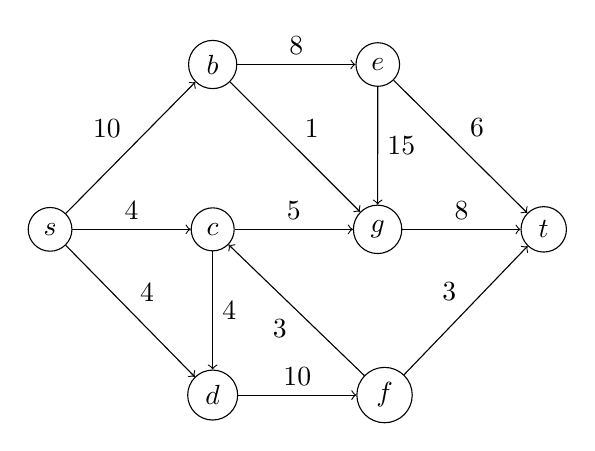
\begin{tikzpicture}
		[vertex/.style={circle, draw=black, node distance=1.5cm}]
		\node[vertex] (s) {\(s\)};
		\node[vertex, right=of s] (c) {\(c\)};
		\node[vertex, above=of c] (b) {\(b\)};
		\node[vertex, below=of c] (d) {\(d\)};
		\node[vertex, right=of b] (e) {\(e\)};
		\node[vertex, right=of d] (f) {\(f\)};
		\node[vertex, right=of c] (g) {\(g\)};
		\node[vertex, right=of g] (t) {\(t\)};

		\draw[->] (s) to["10"] (b);
		\draw[->] (s) to["4"] (c);
		\draw[->] (s) to["4"] (d);
		\draw[->] (c) to["4"] (d);
		\draw[->] (b) to["8"] (e);
		\draw[->] (b) to["1"] (g);
		\draw[->] (e) to["15"] (g);
		\draw[->] (c) to["5"] (g);
		\draw[->] (d) to["10"] (f);
		\draw[->] (f) to["3"] (c);
		\draw[->] (f) to["3"] (t);
		\draw[->] (g) to["8"] (t);
		\draw[->] (e) to["6"] (t);
	\end{tikzpicture}
	\caption{A network}
	\label{q1}
\end{figure}



\end{document}